\newcommand{\ImplementationTitle}{Implementation}
\begin{frame}
    \frametitle{\ImplementationTitle}
    \centering
    \begin{minipage}{1\textwidth}
        \begin{itemize}%[<+->]
            \item Processes
            \begin{itemize}
                \item State machines
            \end{itemize}
            \item Buffers
            \begin{itemize}
                \item Memory segments
                \item Dictionary
            \end{itemize}
            \item Interface signal control
            \begin{itemize}
                \item Buffer-Producer
                \item Compute-Producer
            \end{itemize}
            \item Interface control
            \begin{itemize}
                \item Usage
                \item Limitations
            \end{itemize}
        \end{itemize}
    \end{minipage}
\end{frame}


\begin{frame}[fragile]
    \frametitle{\ImplementationTitle}
    \framesubtitle{Processes}
    State machines\\
    %\begin{onlyenv}<2>
    \begin{minipage}[t]{0.3\textwidth}
        \begin{mintedcsharp}
            public class SomeProcess : StateProcess
            {
              private override async Task OnTickAsync()
              {
                a();
                await ClockAsync();
                b();
                await ClockAsync();
                c();
                await ClockAsync();
              }
            }
        \end{mintedcsharp}
    \end{minipage}%
    %\end{onlyenv}%
    \hfill%
    \begin{minipage}[t]{0.3\textwidth}
        \begin{mintedcsharp}
            public class SomeProcess : SimpleProcess
            {
            // Initial state
            state = A;

            protected override void OnTick()
            {
              switch(state) {
                case A:
                  a();
                  state = B;
                case B:
                  b();
                  state = C;
                case C:
                  c();
                  state = A;
              }
            }
        \end{mintedcsharp}
    \end{minipage}%
    \hfill%
    \begin{minipage}[t]{0.3\textwidth}
        \begin{figure}
                \centering
                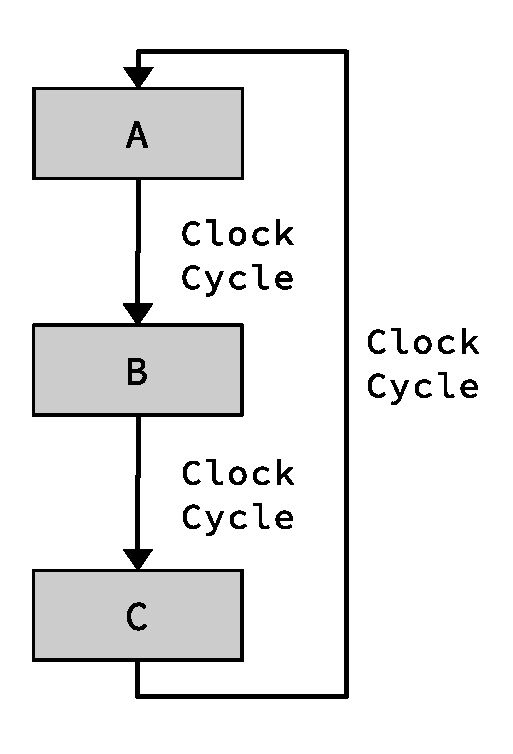
\includegraphics[scale=0.45]{implementation/empty_process_fsm.eps}
        \end{figure}
    \end{minipage}
\end{frame}



\begin{frame}[fragile]
    \frametitle{\ImplementationTitle}
    \framesubtitle{Processes}
    Examples\\
    \begin{minipage}[t]{0.5\textwidth}
        \begin{figure}
                \centering
                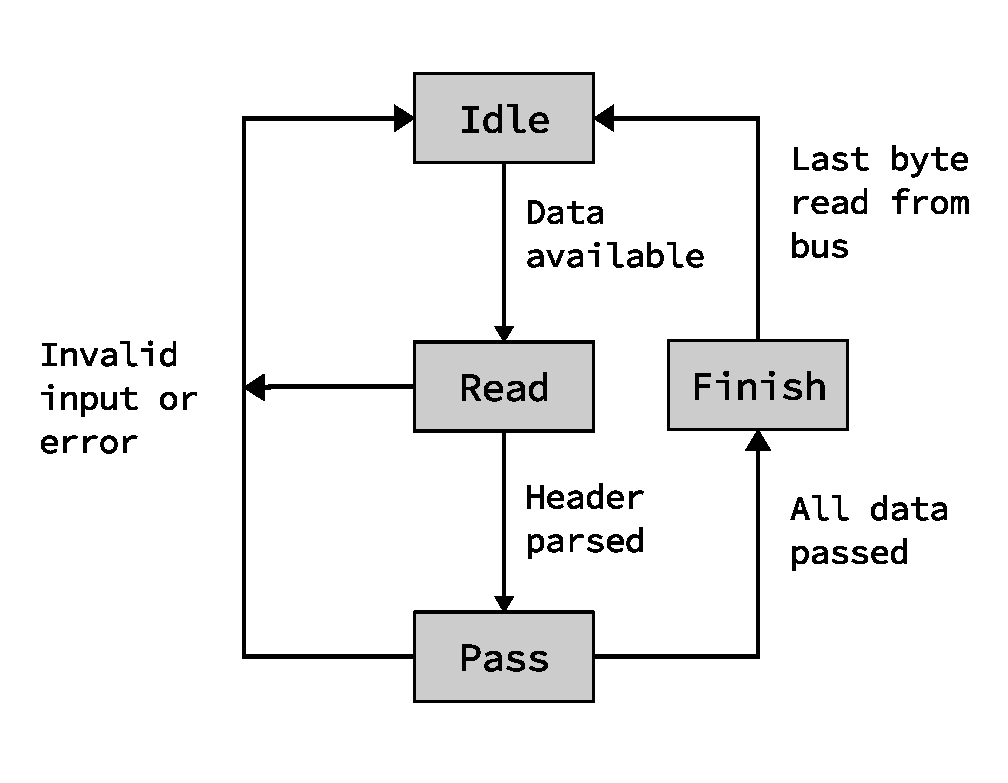
\includegraphics[scale=0.35]{implementation/internet_in_fsm.eps}
        \end{figure}
    \end{minipage}%
    \hfill%
    \begin{minipage}[t]{0.5\textwidth}
        \begin{figure}
                \centering
                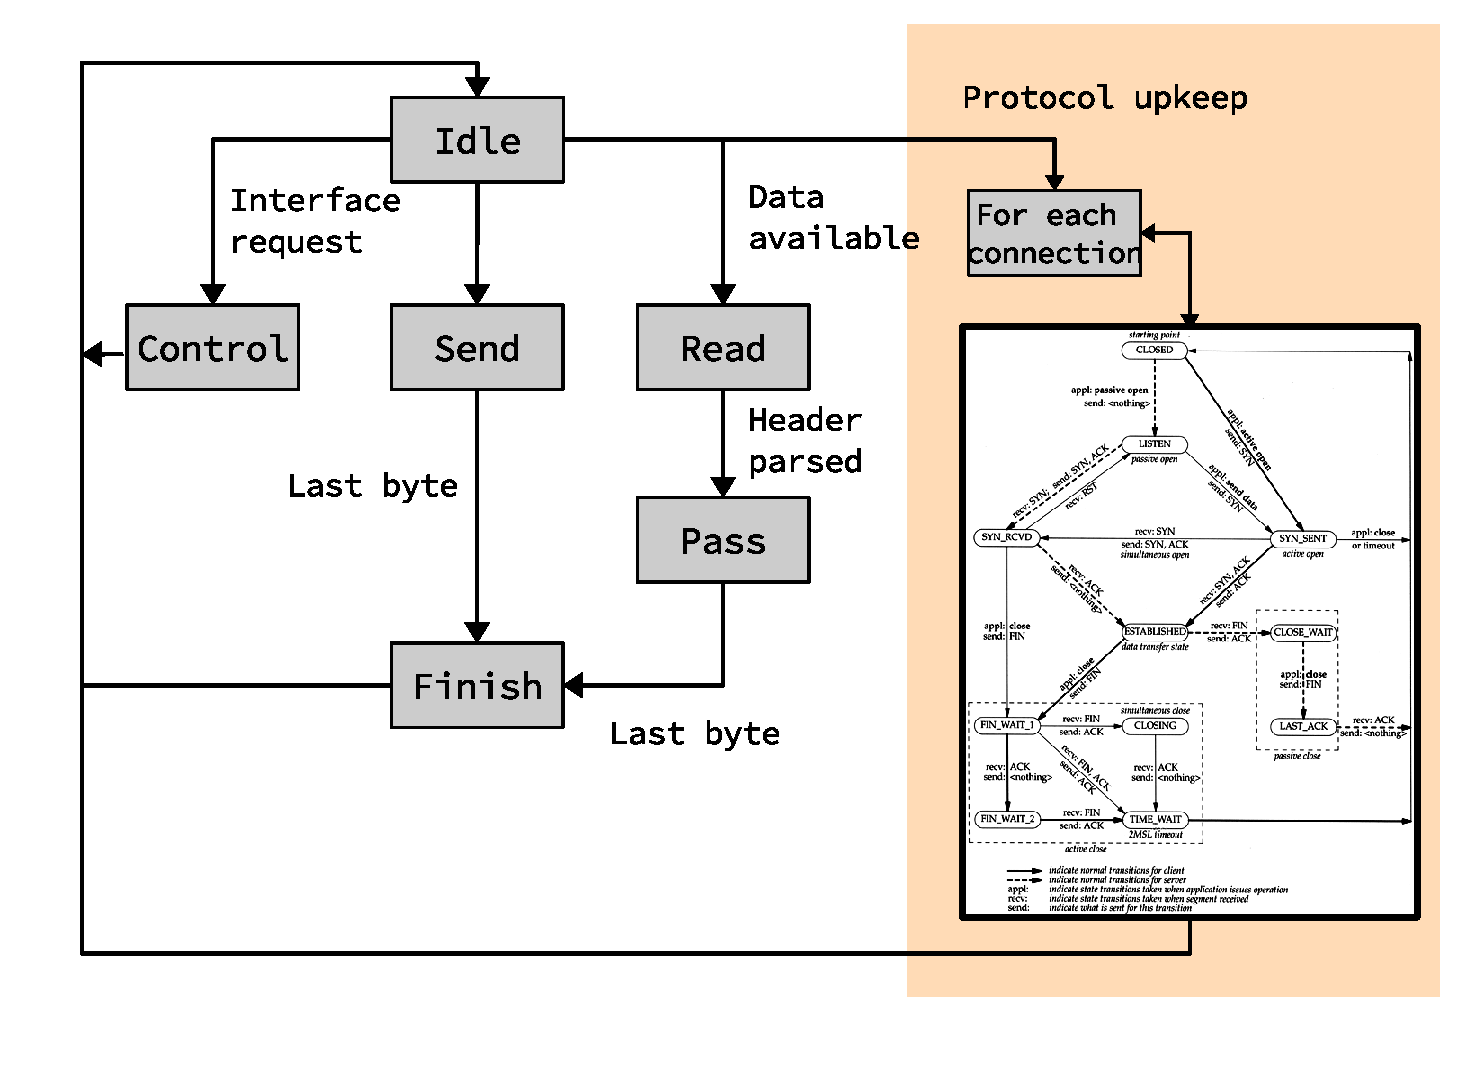
\includegraphics[scale=0.35]{implementation/transport_fsm.eps}
        \end{figure}
    \end{minipage}
\end{frame}


\begin{frame}[fragile]
    \frametitle{\ImplementationTitle}
    \framesubtitle{Buffers}
    Memory segments\\
    \begin{minipage}[t]{1\textwidth}
        \begin{figure}
                \centering
                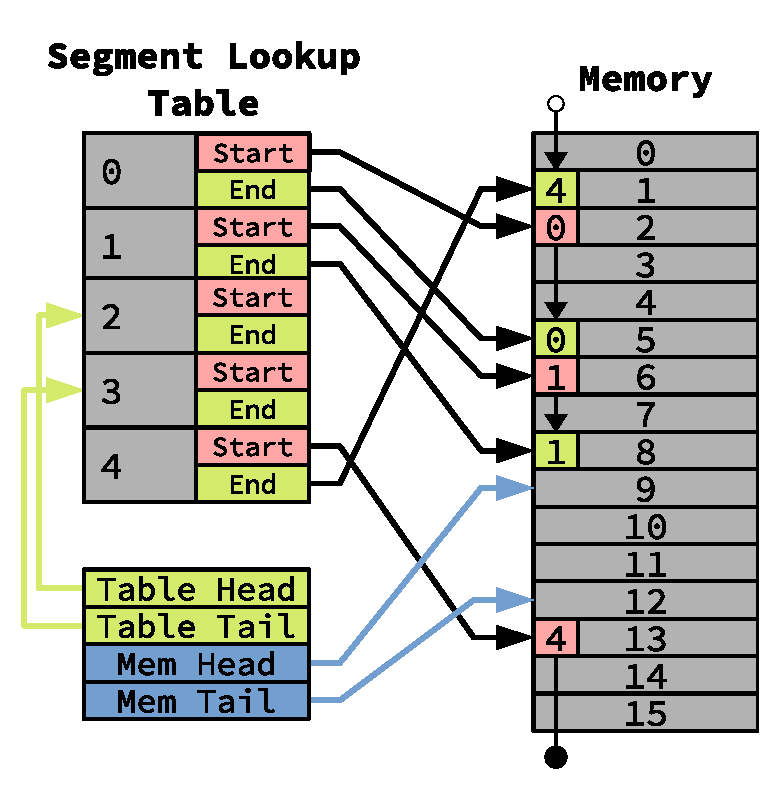
\includegraphics[scale=0.50]{implementation/memory_segments.eps}
        \end{figure}
    \end{minipage}
\end{frame}

\begin{frame}[fragile]
    \frametitle{\ImplementationTitle}
    \framesubtitle{Buffers}
    Memory dictionary\\
    \begin{minipage}[t]{1\textwidth}
        \begin{figure}
                \centering
                \includegraphics[scale=0.60]{implementation/memory_dictionary.eps}
        \end{figure}
    \end{minipage}
\end{frame}



\begin{frame}[fragile]
    \frametitle{\ImplementationTitle}
    \framesubtitle{Interface signal protocol}
    Inspired by AXI4\\
    \begin{columns}
        \begin{column}{0.4\textwidth}
           \begin{itemize}
               \item Single clock offset when sending data.
               \item Indicate end of stream with \texttt{bytes\_left}.
           \end{itemize}
        \end{column}
        \begin{column}{0.5\textwidth}  %%<--- here
            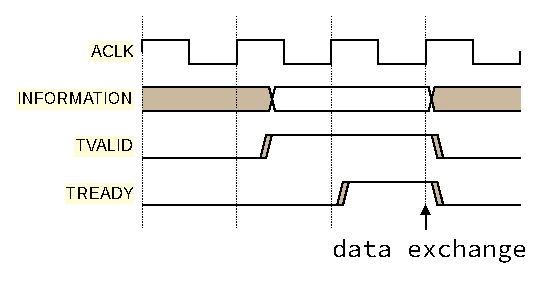
\includegraphics[scale=0.7]{implementation/axi4_handshake.eps}
        \end{column}
    \end{columns}
\end{frame}


\begin{frame}[fragile]
    \frametitle{\ImplementationTitle}
    \framesubtitle{Interface signal protocol}
    \begin{minipage}[t]{0.5\textwidth}
        \begin{figure}
                \centering
                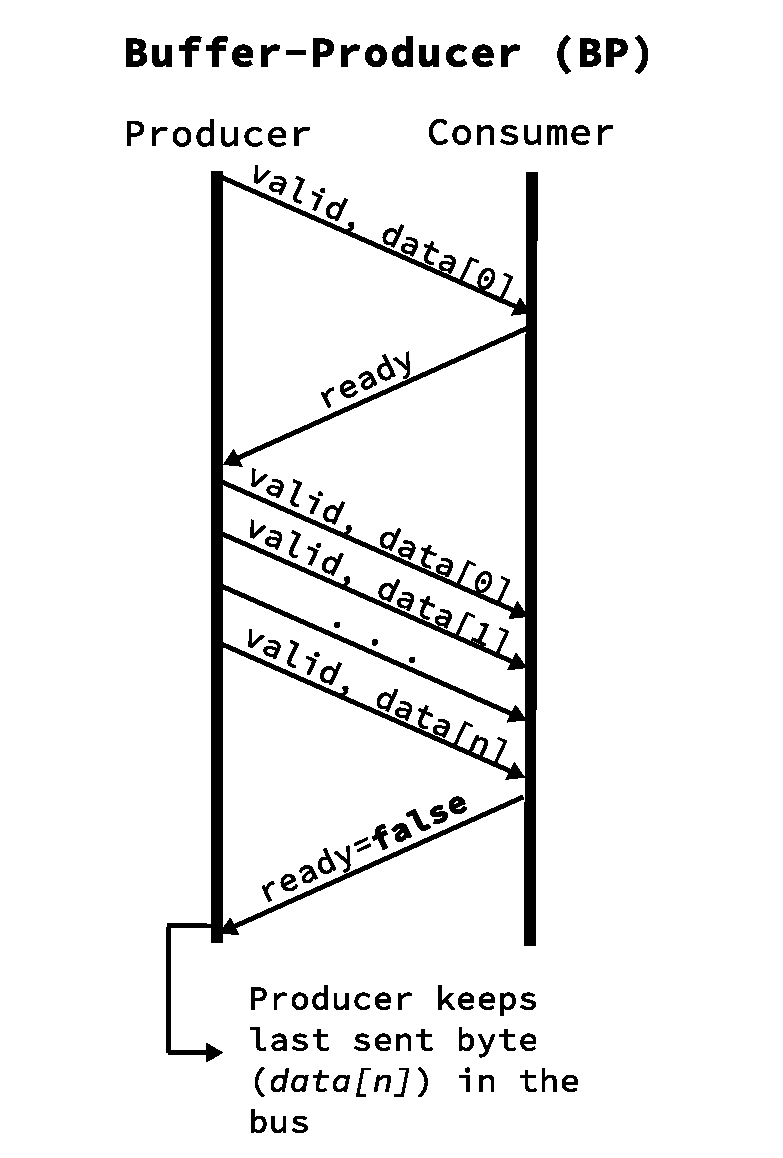
\includegraphics[scale=0.35]{implementation/buffer_producer.eps}
        \end{figure}
    \end{minipage}%
    \hfill%
    \begin{minipage}[t]{0.5\textwidth}
        \begin{figure}
                \centering
                \includegraphics[scale=0.35]{implementation/compute_producer.eps}
        \end{figure}
    \end{minipage}
\end{frame}





\begin{frame}[fragile]
    \frametitle{\ImplementationTitle}
    \framesubtitle{Interface protocol}
    The interface structures\\
    \begin{minipage}[t]{0.4\textwidth}
        \begin{mintedcsharp}
            enum InterfaceFunction : byte
            {
                INVALID = 0,
                // BIND = 1,
                LISTEN = 2,
                CONNECT = 3,
                ACCEPT = 4,
                CLOSE = 7,
                // ...
                OPEN = 255,
            }

            struct InterfaceData
            {
                public int socket;
                public uint ip;
                public byte protocol;
                public ushort port;
            }
        \end{mintedcsharp}
    \end{minipage}%
    \hfill%
    \begin{minipage}[t]{0.4\textwidth}
        \begin{mintedcsharp}
            interface InterfaceBus : IBus
            {
                bool valid;
                byte interface_function;
                InterfaceData request;
            }

            interface InterfaceControlBus : IBus
            {
                bool valid;

                byte exit_status;
                byte interface_function;
                InterfaceData request;
                InterfaceData response;
            }
        \end{mintedcsharp}
    \end{minipage}
\end{frame}


\begin{frame}%[fragile]
    \frametitle{\ImplementationTitle}
    \framesubtitle{Interface protocol}
    Limitations
    \begin{itemize}
        \item One request at a time.
        \item Arbitrary delay between request and response.
    \end{itemize}
\end{frame}
